% --- LaTeX Homework Template - S. Venkatraman ---

% --- Set document class and font size ---

\documentclass[letterpaper, 11pt]{article}

% --- Package imports ---

\usepackage{
  amsmath, amsthm, amssymb, mathtools, dsfont,	  % Math typesetting
  graphicx, wrapfig, subfig, float,                  % Figures and graphics formatting
  listings, color, inconsolata, pythonhighlight,     % Code formatting
  fancyhdr, sectsty, hyperref, enumerate, enumitem } % Headers/footers, section fonts, links, lists

% --- Page layout settings ---

% Set page margins
\usepackage[left=1.35in, right=1.35in, bottom=1in, top=1.1in, headsep=0.2in]{geometry}

% Anchor footnotes to the bottom of the page
\usepackage[bottom]{footmisc}
\usepackage{xcolor}

% Set line spacing
\renewcommand{\baselinestretch}{1}

% Set spacing between paragraphs
\setlength{\parskip}{1.5mm}

% Allow multi-line equations to break onto the next page
\allowdisplaybreaks

% Enumerated lists: make numbers flush left, with parentheses around them
\setlist[enumerate]{wide=0pt, leftmargin=21pt, labelwidth=0pt, align=left}
\setenumerate[1]{label={(\arabic*)}}

% --- Page formatting settings ---

% Set link colors for labeled items (blue) and citations (red)
\hypersetup{colorlinks=true, linkcolor=blue, citecolor=red}

% Make reference section title font smaller
\renewcommand{\refname}{\large\bf{References}}

% --- Settings for printing computer code ---

% Define colors for green text (comments), grey text (line numbers),
% and green frame around code
\definecolor{greenText}{rgb}{0.5, 0.7, 0.5}
\definecolor{greyText}{rgb}{0.5, 0.5, 0.5}
\definecolor{codeFrame}{rgb}{0.5, 0.7, 0.5}

% Define code settings
\lstdefinestyle{code} {
  frame=single, rulecolor=\color{codeFrame},            % Include a green frame around the code
  numbers=left,                                         % Include line numbers
  numbersep=8pt,                                        % Add space between line numbers and frame
  numberstyle=\tiny\color{greyText},                    % Line number font size (tiny) and color (grey)
  commentstyle=\color{greenText},                       % Put comments in green text
  basicstyle=\linespread{1.1}\ttfamily\footnotesize,    % Set code line spacing
  keywordstyle=\ttfamily\footnotesize,                  % No special formatting for keywords
  showstringspaces=false,                               % No marks for spaces
  xleftmargin=1.95em,                                   % Align code frame with main text
  framexleftmargin=1.6em,                               % Extend frame left margin to include line numbers
  breaklines=true,                                      % Wrap long lines of code
  postbreak=\mbox{\textcolor{greenText}{$\hookto$}\space} % Mark wrapped lines with an arrow
}

% Set all code listings to be styled with the above settings
\lstset{style=code}

% --- Math/Statistics commands ---

% Add a reference number to a single line of a multi-line equation
% Usage: "\numberthis\label{labelNameHere}" in an align or gather environment
\newcommand\numberthis{\addtocounter{equation}{1}\tag{\theequation}}

% Shortcut for bold text in math mode, e.g. $\b{X}$
\let\b\mathbf

% Shortcut for bold Greek letters, e.g. $\bg{\beta}$
\let\bg\boldsymbol

% Shortcut for calligraphic script, e.g. %\mc{M}$
\let\mc\mathcal

% \mathscr{(letter here)} is sometimes used to denote vector spaces
\usepackage[mathscr]{euscript}

% Convergence: right arrow with optional text on top
% E.g. $\converge[w]$ for weak convergence
\newcommand{\converge}[1][]{\xto{#1}}

% Normal distribution: arguments are the mean and variance
% E.g. $\normal{\mu}{\sigma}$
\newcommand{\normal}[2]{\mathcal{N}\left(#1,#2\right)}

% Uniform distribution: arguments are the left and right endpoints
% E.g. $\unif{0}{1}$
\newcommand{\unif}[2]{\text{Uniform}(#1,#2)}

% Independent and identically distributed random variables
% E.g. $ X_1,...,X_n \iid \normal{0}{1}$
\newcommand{\iid}{\stackrel{\smash{\text{iid}}}{\sim}}

% Equality: equals sign with optional text on top
% E.g. $X \equals[d] Y$ for equality in distribution
\newcommand{\equals}[1][]{\stackrel{\smash{#1}}{=}}

% Math mode symbols for common sets and spaces. Example usage: $\R$
\newcommand{\R}{\mathbb{R}}   % Real numbers
\newcommand{\C}{\mathbb{C}}   % Complex numbers
\newcommand{\Q}{\mathbb{Q}}   % Rational numbers
\newcommand{\Z}{\mathbb{Z}}   % Integers
\newcommand{\N}{\mathbb{N}}   % Natural numbers
\newcommand{\F}{\mathcal{F}}  % Calligraphic F for a sigma algebra
\newcommand{\El}{\mathcal{L}} % Calligraphic L, e.g. for L^p spaces

% Math mode symbols for probability
\newcommand{\pr}{\mathbb{P}}    % Probability measure
\newcommand{\E}{\mathbb{E}}     % Expectation, e.g. $\E(X)$
\newcommand{\var}{\text{Var}}   % Variance, e.g. $\var(X)$
\newcommand{\cov}{\text{Cov}}   % Covariance, e.g. $\cov(X,Y)$
\newcommand{\corr}{\text{Corr}} % Correlation, e.g. $\corr(X,Y)$
\newcommand{\B}{\mathcal{B}}    % Borel sigma-algebra

% Other miscellaneous symbols
\newcommand{\tth}{\text{th}}	% Non-italicized 'th', e.g. $n^\tth$
\newcommand{\Oh}{\mathcal{O}}	% Big-O notation, e.g. $\O(n)$
\newcommand{\1}{\mathds{1}}	% Indicator function, e.g. $\1_A$

% Additional commands for math mode
\DeclareMathOperator*{\argmax}{argmax}    % Argmax, e.g. $\argmax_{x\in[0,1]} f(x)$
\DeclareMathOperator*{\argmin}{argmin}    % Argmin, e.g. $\argmin_{x\in[0,1]} f(x)$
\DeclareMathOperator*{\spann}{Span}       % Span, e.g. $\spann\{X_1,...,X_n\}$
\DeclareMathOperator*{\bias}{Bias}        % Bias, e.g. $\bias(\hat\theta)$
\DeclareMathOperator*{\ran}{ran}          % Range of an operator, e.g. $\ran(T) 
\DeclareMathOperator*{\dv}{d\!}           % Non-italicized 'with respect to', e.g. $\int f(x) \dv x$
\DeclareMathOperator*{\diag}{diag}        % Diagonal of a matrix, e.g. $\diag(M)$
\DeclareMathOperator*{\trace}{trace}      % Trace of a matrix, e.g. $\trace(M)$

% Numbered theorem, lemma, etc. settings - e.g., a definition, lemma, and theorem appearing in that 
% order in Section 2 will be numbered Definition 2.1, Lemma 2.2, Theorem 2.3. 
% Example usage: \begin{theorem}[Name of theorem] Theorem statement \end{theorem}
\theoremstyle{definition}
\newtheorem{theorem}{Theorem}[section]
\newtheorem{proposition}[theorem]{Proposition}
\newtheorem{lemma}[theorem]{Lemma}
\newtheorem{corollary}[theorem]{Corollary}
\newtheorem{definition}[theorem]{Definition}
\newtheorem{example}[theorem]{Example}
\newtheorem{remark}[theorem]{Remark}

% Un-numbered theorem, lemma, etc. settings
% Example usage: \begin{lemma*}[Name of lemma] Lemma statement \end{lemma*}
\newtheorem*{theorem*}{Theorem}
\newtheorem*{proposition*}{Proposition}
\newtheorem*{lemma*}{Lemma}
\newtheorem*{corollary*}{Corollary}
\newtheorem*{definition*}{Definition}
\newtheorem*{example*}{Example}
\newtheorem*{remark*}{Remark}
\newtheorem*{claim}{Claim}

% --- Left/right header text (to appear on every page) ---

% Include a line underneath the header, no footer line
\pagestyle{fancy}
\renewcommand{\footrulewidth}{0pt}
\renewcommand{\headrulewidth}{0.4pt}

% Left header text: course name/assignment number
\lhead{Statistics - Assignment 1}

% Right header text: your name
\rhead{Zian Gong}

% --- Document starts here ---

\begin{document}

\textbf{Problem 1}

(a)

\begin{align*}
    \Gamma(\alpha+1) & = \int_{0}^{\infty } u^{\alpha} e^{-u} \, du                                                            \\
                     & = - \int_{0}^{\infty} u^{\alpha} \, de^{-u}                                                             \\
                     & = - \Big[u^{\alpha}e^{-u}\Big|_0^{\infty }- \int_{0}^{\infty } \alpha u^{\alpha - 1} e^{-u}  \, du\Big] \\
                     & = -\Big[ 0- 0- \alpha \int_{0}^{\infty } u^{\alpha-1}e^{-u} \, du \Big]                                 \\
                     & =  \alpha \int_{0}^{\infty } u^{\alpha-1}e^{-u} \, du = \alpha \Gamma(\alpha)
\end{align*}


(b)

\begin{align*}
                    & f_X(x;\alpha,\lambda) \geq  0, \forall x > 0                                                                                                                          \\
                    & F_X(t;\alpha,\lambda) = \int_{0}^{t} f_x(x;\alpha,\lambda) \, dx = \frac{1}{\Gamma(\alpha)} \int_{0}^{t} (\lambda x)^{\alpha - 1} \exp ^{-\lambda x}  \, d(\lambda x) \\
    \Longrightarrow & F_X(0;\alpha,\lambda) = 0 \text{ and }  F_X(\infty ;\alpha,\lambda) = 1
\end{align*}

(c)

$f_X(x;1.5,1) = \frac{1}{\Gamma(1.5)}x^\frac{1}{2}\exp(-x), \, x>0$ \[
    f_X'(x;1.5,1) = (\frac{1}{2}x^{-\frac{1}{2}}-x^{\frac{1}{2}})e^{-x}
\]

$f_X(x;3,1) = \frac{1}{\Gamma(3)}x^2\exp(-x), \, x>0$ \[
    f_X'(x;3,1) = x(2-x)e^{-x}
\]

The shapes of two pdfs are shown in Figure \ref{fig:p1-c}

\begin{figure}[H] % h=here, t=top, b=bottom, p=page
    \centering
    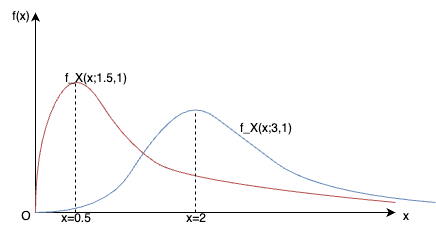
\includegraphics[width=0.75\textwidth]{images/stats-a1-p1-c.drawio.png}
    \caption{Problem 1-(c)}
    \label{fig:p1-c}
\end{figure}


(d)

For $\alpha = 1$, then the pdf is \[
    f_X(x;\lambda) = \lambda\exp(-\lambda x) \, \lambda > 0
\]
The expectation is given by, where $\Gamma(1) = \int_{0}^{\infty } \exp(-u) \, du = 1 $ \begin{align*}
    E(X) & = \int_{0}^{\infty } xf_X(x;\lambda) \, dx                                                \\
         & = \int_{0}^{\infty } x\lambda\exp(-\lambda x) \, dx                                       \\
         & = - \Big[ xe^{-\lambda x} \Big|_0^\infty  - \int_{0}^{\infty } e^{-\lambda x} \, dx \Big] \\
         & = \frac{1}{\lambda} \int_{0}^{\infty } \exp(-\lambda x) \, d(\lambda x) = 1/\lambda       \\
\end{align*}
The variance is given by \begin{align*}
    Var(X) & = \int_{0}^{\infty } (x- \frac{1}{\lambda})^{2}f_X(x ; \lambda) \, dx                                                                                                                              \\
           & = \int_{0}^{\infty } (x- \frac{1}{\lambda})^{2} \lambda\exp(-\lambda x) \, dx                                                                                                                      \\
           & = \lambda\Big[\int_{0}^{\infty } x^2 \exp(-\lambda x) \, dx -\frac{2}{\lambda}\int_{0}^{\infty } x \exp(-\lambda x) \, dx + \frac{1}{\lambda ^{2}} \int_{0}^{\infty } \exp(-\lambda x) \, dx \Big] \\
           & = \lambda \Big[ \frac{2}{\lambda} \int_{0}^{\infty } x e^{-\lambda x} \, dx  - \frac{2}{\lambda} \int_{0}^{\infty } x e^{-\lambda x} \, dx + \frac{1}{\lambda ^{2}} \frac{1}{\lambda} \Big]        \\
           & = \frac{1}{\lambda ^{2}}
\end{align*}

(e)
\begin{align*}
     & m(t) = E(e^{tx}) = \int_{0}^{\infty } e^{tx} f_X(x;\alpha,\lambda) \, dx                                                                                                                  \\
     & \frac{d m(t)}{dt} = \int_{0}^{\infty } xe^{tx}f_X(x;\alpha,\lambda) \, dx \Longrightarrow \frac{d m(t)}{dt}\Big|_{x=0} = \int_{0}^{\infty } xf_X(x;\alpha,\lambda) \, dx = E(x)           \\
     & \frac{d^2 m(t)}{dt^2} = \int_{0}^{\infty } x^2e^{tx}f_X(x;\alpha,\lambda) \, dx \Longrightarrow \frac{d m(t)}{dt}\Big|_{x=0} = \int_{0}^{\infty } x^2f_X(x;\alpha,\lambda) \, dx = E(x^2) \\
\end{align*}

\bigskip
\hrule
\bigskip


\textbf{Problem 2}

(a)

pdf:
\[
    f(x) = p_1 \frac{1}{\sigma_1} \phi (\frac{x - \mu_1}{\sigma_1}) + p_2 \frac{1}{\sigma_2} \phi (\frac{x - \mu_2}{\sigma_2})
\]

(b)

Expectation: \begin{align*}
    E(X) & = \int_{-\infty }^{\infty } xf(x) \, dx = \int_{-\infty }^{\infty } p_1 x\frac{1}{\sigma_1} \phi (\frac{x - \mu_1}{\sigma_1}) + p_2 x\frac{1}{\sigma_2} \phi (\frac{x - \mu_2}{\sigma_2})  \, dx \\
         & = p_1 \mu_2 + p_2 \mu_2
\end{align*}

Variance: \begin{align*}
     & var(X) = E(X^2) - [E(X)]^2                                                                                                                                                                                                              \\
     & =   \int_{-\infty }^{\infty } x^2f(x) \, dx = \int_{-\infty }^{\infty } p_1 x^2\frac{1}{\sigma_1} \phi (\frac{x - \mu_1}{\sigma_1}) + p_2 x^2\frac{1}{\sigma_2} \phi (\frac{x - \mu_2}{\sigma_2})  \, dx - ( p_1 \mu_2 + p_2 \mu_2)^{2} \\
\end{align*}
Since \begin{align*}
     & \int_{-\infty }^{\infty } x^2\frac{1}{\sigma_1} \phi (\frac{x - \mu_1}{\sigma_1})                                                                                                                                                                                                        \\
     & = \int_{-\infty }^{\infty } (x-\mu_1)^{2}\frac{1}{\sigma_1} \phi (\frac{x - \mu_1}{\sigma_1})\, dx + 2\int_{-\infty }^{\infty } x\mu_1\frac{1}{\sigma_1} \phi (\frac{x - \mu_1}{\sigma_1}) - \int_{-\infty }^{\infty } \mu_1^2 \frac{1}{\sigma_1} \phi (\frac{x - \mu_1}{\sigma_1})\, dx \\
     & = \sigma_1^2 + 2 \mu_1^{2} - \mu_1^2 = \sigma_1^2 + \mu_1^{2}
\end{align*}
Similarly, $\int_{-\infty }^{\infty } x^2\frac{1}{\sigma_2} \phi (\frac{x - \mu_2}{\sigma_2}) = \sigma_2^2 + \mu_2^2$.

Thus, \[
    var(X) = p_1(\sigma_1^2 + \mu_1 ^{2}) + p_2( \sigma_2^2 + \mu_2^2) - ( p_1 \mu_2 + p_2 \mu_2)^{2}
\]



(c)

When $\sigma_1 = \sigma_2 = 1, p_1 = p_2 = \frac{1}{2}, \mu_1 + \mu_2 = 0$, the pdf can be written as:
\[
    f(x) = \frac{1}{2}  \phi ({x - \mu_1}) + \frac{1}{2} \phi ({x + \mu_1})
\]
we have $f(-x) = f(x)$, so it is symmetric. Figure \ref{fig:p2-c}

\begin{figure}[H] % h=here, t=top, b=bottom, p=page
    \centering
    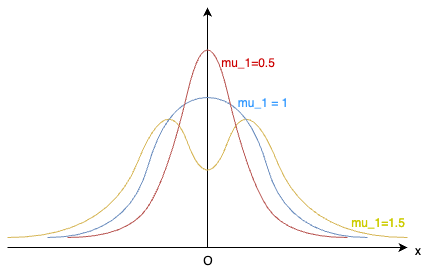
\includegraphics[width=0.75\textwidth]{images/stats-a1-p2-c.drawio.png}
    \caption{Problem 2-(c)}
    \label{fig:p2-c}
\end{figure}

\bigskip
\hrule
\bigskip


\textbf{Problem 3}

(a)

\[
    \sum_{x=0}^{\infty } P(X=x) = \sum_{x=0}^{\infty } e^{-\lambda}\lambda^{x}/x! = e^{-\lambda} \sum_{x=0}^{\infty }\lambda^x/x!
\]
Since $e^\lambda = 1 + \lambda + \frac{\lambda ^{2}}{2!} + \frac{\lambda ^{3}}{3!} + \dots$, replace it into the equation \[
    \sum_{x=0}^{\infty } P(X=x) =  e^{-\lambda}  e^{\lambda} = 1
\]

Expectation \begin{align*}
    E(X) & = \sum_{x=0}^{\infty } xP(X=x) = \sum_{x=0}^{\infty } x e^{-\lambda}\lambda^{x}/x! = \lambda \sum_{x=1}^{\infty } e^{-\lambda}\lambda^{x -1}/(x-1)! \\
         & = \lambda
\end{align*}

Variance \begin{align*}
    Var(X) & = \sum_{x=0}^{\infty } (x-\lambda)^{2} P(X=x) = \sum_{x=0}^{\infty } (x-\lambda)^{2}  e^{-\lambda}\lambda^{x}/x! \\
           & = \sum_{x=0}^{\infty } x ^{2} e^{-\lambda}\lambda^{x}/x!
    -2 \lambda\sum_{x=0}^{\infty } x  e^{-\lambda}\lambda^{x}/x!
    + \lambda ^{2} \sum_{x=0}^{\infty } e^{-\lambda}\lambda^{x}/x!                                                            \\
           & = \lambda \sum_{x=1}^{\infty } x e^{-\lambda}\lambda^{x-1}/(x-1)! -2\lambda \cdot \lambda + \lambda ^{2}         \\
           & = \lambda e^{-\lambda} (e^{\lambda} + \lambda e^{\lambda}) - \lambda ^{2}                                        \\
           & = \lambda
\end{align*}

(b)

\[
    m(t) = E(e^{xt}) =  \sum_{x=0}^{\infty } e^{xt - \lambda}\lambda^{x}/x!
\]
\[
    \kappa(t) = \ln m(t) = \ln \Big[ \sum_{x=0}^{\infty } e^{xt - \lambda}\lambda^{x}/x! \Big]
\]
We have $m(0) = \sum_{x=0}^{\infty } e^{- \lambda}\lambda^{x}/x! = 1$.
\[
    \frac{d \kappa(t)}{dt} = \frac{m'(t)}{m(t)} \Longrightarrow  \frac{d \kappa(t)}{dt}\Big|_{t=0} = \frac{m'(0)}{m(0)} = m'(0) = \sum_{x=0}^{\infty }x e^{xt - \lambda}\lambda^{x}/x! = E(X)
\]
\begin{align*}
     & \frac{d^2 \kappa(t)}{dt^2} = \frac{m''(t)m(t) - m'(t)m'(t)}{[m(t)]^{2}}                                \\
     & \Longrightarrow  \frac{d^2 \kappa(t)}{dt^2}\Big|_{t=0} = m''(0) -[ m'(0)]^{2} =  m''(0) - [E(X)]^{2}   \\
     & = \sum_{x=0}^{\infty } x^2 e^{xt - \lambda}\lambda^{x}/x! - [E(X)]^{2}  = E(X^2) - [E(X)]^{2} = var(X)
\end{align*}

\bigskip
\hrule
\bigskip

\textbf{Problem 7}

pdf
\[
    f_X(x) = \left\{\begin{array}{l}
        \frac{1}{2}, x \in [-1,1] \\
        0, x \notin [-1,1]        \\
    \end{array}\right.
\]

cdf \[
    F_X(x) = \left\{\begin{array}{l}
        0, x < -1                      \\
        \frac{1}{2}(x+1), x \in [-1,1] \\
        1, x > 1
    \end{array}\right.
\]

(a)

\[
    Y = \left| X \right| \Longrightarrow X = \pm Y
\]

\[
    f_Y(y) = f_X(y) + f_X(-y) = 1
\]

Then pdf \[
    f_Y = \left\{\begin{array}{l}
        1, y \in [0,1]    \\
        0, y \notin [0,1] \\
    \end{array}\right.
\]
and cdf \[
    F_Y = \left\{\begin{array}{l}
        0, y < 0       \\
        y, y \in [0,1] \\
        1, y > 1
    \end{array}\right.
\]
expectation: \[
    E(X) = \int_{0}^{1} y \, dy = \frac{1}{2}
\]


\bigskip
\hrule
\bigskip

\textbf{Problem 22}

(a)

\[
    f(-1) + f(0) + f(1) = \frac{4}{c} + \frac{1}{c} + \frac{4}{c} = 1 \Longrightarrow c = 9
\]

(b)

\[
    M(t) = \frac{4}{9} e^{-t} + \frac{1}{9} + \frac{4}{9} e^t
\]

(c)

Mean: \[
    \frac{dM(t)}{dt}\Big|_{t=0}= - \frac{4}{9} + \frac{4}{9} = 0
\]

Variance: \[
    \frac{d^2M(t)}{dt^2}\Big|_{t=0} = \frac{4}{9} + \frac{4}{9}  = \frac{8}{9}
\]

% --- Document ends here ---

\end{document}

